% main tex file

% begin ACM TAPS stuff
\documentclass[sigconf]{acmart}
\usepackage{xspace}
\usepackage{hyperref}

%%
%% \BibTeX command to typeset BibTeX logo in the docs
\AtBeginDocument{%
  \providecommand\BibTeX{{%
    \normalfont B\kern-0.5em{\scshape i\kern-0.25em b}\kern-0.8em\TeX}}}

%% Rights management information.  This information is sent to you
%% when you complete the rights form.  These commands have SAMPLE
%% values in them; it is your responsibility as an author to replace
%% the commands and values with those provided to you when you
%% complete the rights form.
\setcopyright{acmcopyright}
\copyrightyear{2023}
\acmYear{2023}
\acmDOI{XXXXXXX.XXXXXXX}

%% These commands are for a PROCEEDINGS abstract or paper.
% \acmConference[Conference acronym 'XX]{Make sure to enter the correct
%   conference title from your rights confirmation emai}{June 03--05,
%   2018}{Woodstock, NY}
% \acmPrice{15.00}
% \acmISBN{978-1-4503-XXXX-X/18/06}

% end ACM TAPS stuff

% my own stuff
\usepackage{xac}

\newcommand{\xin}[0]{{\texttt{X-index} \xspace}}

\begin{document}

% \title{HCI Papers Are Increasingly Cited More Often by HCI Papers}
\title{HCI Papers Cite HCI Papers, Increasingly So}

\author{Xiang `Anthony' Chen}
\affiliation{%
 \institution{UCLA HCI Research}
 \country{}
}
\email{xac@ucla.edu}

%%
%% By default, the full list of authors will be used in the page
%% headers. Often, this list is too long, and will overlap
%% other information printed in the page headers. This command allows
%% the author to define a more concise list
%% of authors' names for this purpose.
\renewcommand{\shortauthors}{Chen}



%%
%% The abstract is a short summary of the work to be presented in the
%% article.
\begin{abstract}
  We propose \xin---the proportion of papers' citations coming from outside their research field---and use this metric to analyze citations of CHI, UIST, and CSCW papers between 2010 and 2022.
We found an overall decreasing \xin by several measures, indicating that HCI papers have been more and more likely to be cited by HCI papers rather than by non-HCI papers.
\end{abstract}


\ccsdesc[500]{Human-centered computing}

%%
%% Keywords. The author(s) should pick words that accurately describe
%% the work being presented. Separate the keywords with commas.
\keywords{HCI, Citation Metrics, Discipline, Impact}

%% A "teaser" image appears between the author and affiliation
%% information and the body of the document, and typically spans the
%% page.
% \begin{teaserfigure}
%   \includegraphics[width=\textwidth]{figures/sampleteaser}
%   \caption{Seattle Mariners at Spring Training, 2010.}
%   \Description{Enjoying the baseball game from the third-base
%   seats. Ichiro Suzuki preparing to bat.}
%   \label{fig:teaser}
% \end{teaserfigure}

%%
%% This command processes the author and affiliation and title
%% information and builds the first part of the formatted document.
\maketitle

\section{Introduction}

% PROMISE
% you are working in the area of X: what promises does X make to the world? why is X exciting enough for people to care?
% The recent development of \xx promises to [make the world a better place] \xxx
Human-Computer Interaction (HCI) is often considered as one of the most interdisciplinary research fields.
% 
% PROBLEM
% but in order to realize X's promise, we have to solve a key problem ...
% However, the problem is \xxx
Thus we hypothesize that HCI papers must have impact beyond HCI, which can be indicated by how often an HCI paper is cited by non-HCI papers.
% , \ie have forward-citation sources across disciplinary.
% 
% PRIOR WORK
% what is the closet related work to your research? how do you differentiate from them? what is the gap in past work?
% To solve this problem, past work has \xxx
Unfortunately, conventional citation metrics, such as h-index or i-10-index, cannot indicate such impact because they only count the number of citations but not the sources of citations.

% PROPOSED SOLUTION
% summarize your research in one sentence
% To fill in this gap, we design and implement \xxx
% use an example (and refer to figure 1) to walkthrough your research in more details
% As shown in \fgref{fig1}, \xxx
To address this, we propose \xin---a simple metric that measures how often a paper's citations cross the disciplinary boundaries.
Given a set of venues representing a specific research field, X-index is defined as the proportion of citations {\it not} coming these venues.

\xac{todo: briefly describe dataset}

\xac{todo: summarize findings}

\xac{todo: show github link}

% PROOF
% what experiments/evaluations/studies have you run to prove that your idea works?
% To validate \xx, we conducted \xxx


% CONTRIBUTION
% {\bf The main contribution} of this paper is \xxx
% differentiate from prior work
% In contrast to prior work that \xxx
\section{Data}

\subsection{Core HCI Venues}
% 
To calculate HCI's \xin, we first need to define what is considered an HCI paper so that we can know which are HCI \vs non-HCI citations.
To the best of our knowledge, there is no existing `catalog' of all HCI venues that publish HCI papers.
Thus we refer to two sources to compile a list of core HCI venues: the SIGCHI-(co)sponsored conferences \cite{Upcoming19:online} and Google Scholar's top publications under the ``Engineering \& Computer Science - Human Computer Interaction'' category \cite{HumanCom38:online}.

Table \ref{tb:venues} shows the resultant core HCI venues\footnote{Some venues changed their name at some point, thus we at times included multiple identifiers for the same venue.}. For each venue, we manually extract a subset of words from its official name to serve as unique identifier, which we later use in keyword-matching to determine whether a citation is HCI or not.

Admittedly, what is not in this list is not necessarily ``non-HCI''; it is just not included by the two sources we chose.
Nonetheless, we argue that this list approximates the ``boundary'' between HCI and the non-HCI world.
The more we see citations of an HCI paper coming outside of this list (\ie higher \xin), the more likely this HCI paper is having an impact across this ``boundary''.
We refer to papers published outside of this list as `non-HCI papers'.

\begin{table}
    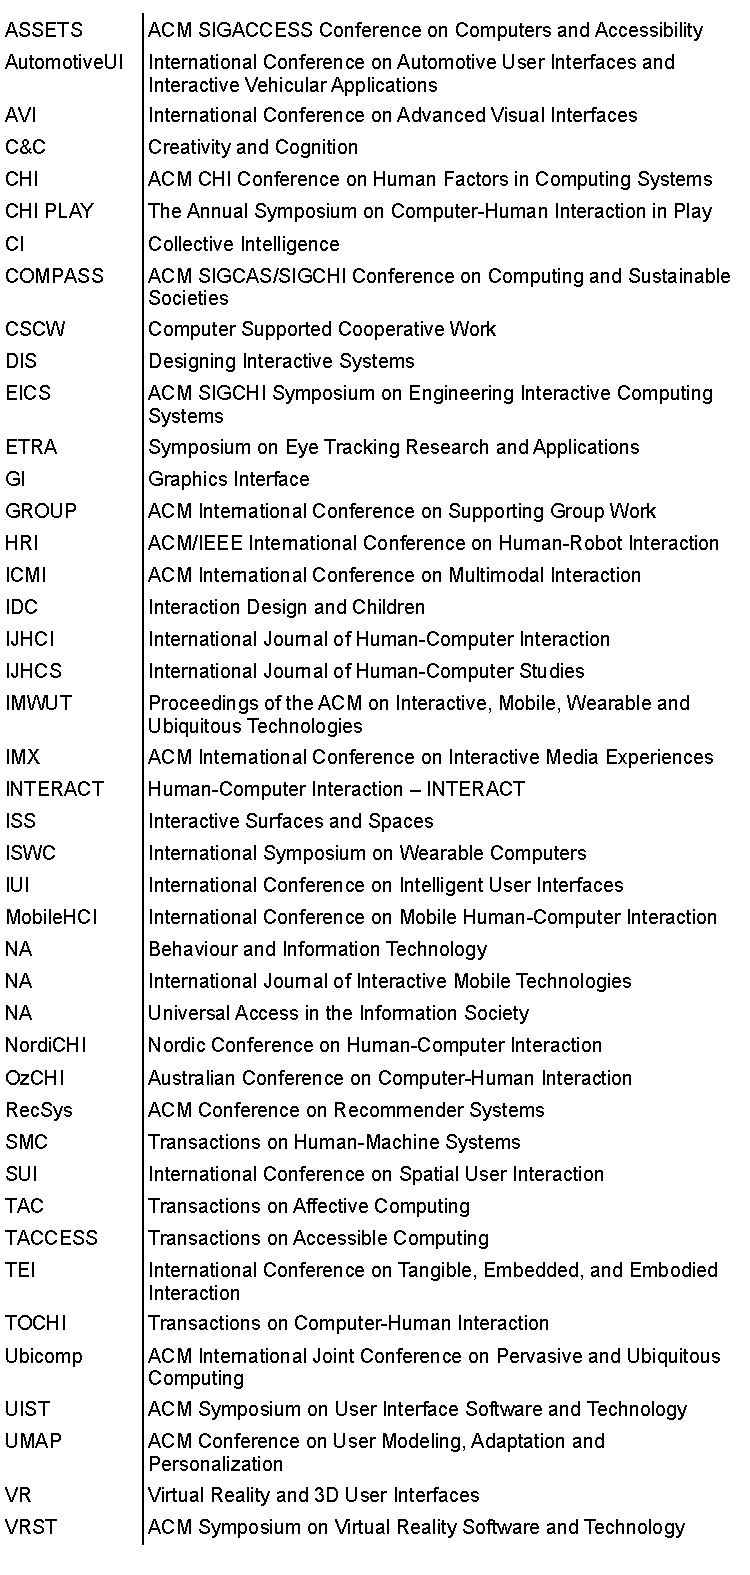
\includegraphics[width=\columnwidth]{figures/hci_venues.pdf}
    \caption{A list of core HCI venues.}
    \label{tb:venues}
\end{table}

\subsection{Citations of CHI, UIST, and CSCW Papers}
% 
Next, we collected DOI data of CHI, UIST and CSCW papers between 2010 to 2020\footnote{Except for CSCW 2020 papers, which the website did not provide.} from the ``What The HCI'' \cite{WhatTheH50:online} website maintained by Kashyap Todi.
We chose CHI, UIST and CSCW because they are three of the most well-recognized HCI venues---we hereafter refer to papers published in these three venues as ``HCI papers''
\footnote{Another reason for selecting these three venues is due to convenience because their data was readily available from \cite{WhatTheH50:online}.}.
It is certainly possible to acquire DOI data of other HCI venues (\eg TOCHI) from other sources (\eg ACM Digital Library).


Then, we port the DOI data into the Citation Chaser app \cite{citation47:online} developed by Neal Haddaway, which uses the Lens.org API \cite{TheLensF23:online} to retrieve citations of a paper based on its DOI.
All the citation data was in the \texttt{.ris} format and collected in January 2023.
We did find that this API did not seem top find all the citations---the total count was smaller than Google Scholar's.
Thus it is best thought of as a sampling, rather than an exhaustive retrieval, of papers' citations. 
We do not believe such a caveat invalidates the subsequent \xin calculation unless the missing citations were biased (\eg missing citations mostly came from just HCI venues).

% (forward) citations
% bib
\section{Analyses \& Findings}

Given a set of papers' citations (total number $N$), we count the number ($n_\text{HCI}$) of citations that came from one of our core HCI venues.
Then, \xin is simply $1-n_\text{HCI}/N$.
Specifically, for a paper that cites an HCI paper, we use simple keyword matching to determine whether that paper belongs to our list of core HCI venues.

\subsection{\xin~ of HCI Papers Published Over the Years}
We calculate the \xin of each year's HCI papers (\eg 11 years of UIST papers between 2010 and 2020), as shown in \fgref{fig1}.
Each point in \fgref{fig1} is the \xin value based on citations of that year's published HCI papers up to when the data was collected (January 2023).
We can see that all three HCI venues' papers have an decreasing \xin over the years.
In other words, HCI papers published later tended to be cited less often by papers outside of the core HCI venues.

One might question that, since citation count is also a function of time, the more recent HCI papers might be disadvantaged simply because they have not existed long enough to attract citations.
To resolve this doubt, we perform the next analysis.

\fg{fig1}{fig1}{1.0}{.}

\subsection{\xin of HCI Papers in the Five Years After Publication}
% One issue of the above analysis is that HCI papers published later (\eg 2019) likely have fewer citations than the earlier ones (\eg 2010) simply because the earlier-published papers existed for a longer period of time.
To balance the playing field, we now consider citations that occurred only within the first five years after an HCI paper was published.
For example, for CHI 2015 papers, we only consider citations of them that occurred between 2016 and 2020.
This constraint narrows us down to only HCI papers published from 2010 to 2017 because, later than that, our data (collected in January 2023) has less than five years of citation information.

As shown in \fgref{fig2}, the result indicates that, even accounting for how long an HCI paper has been around, the overall \xin still seems to decrease over the years.

\fg{fig2}{fig2}{1.0}{.}

\subsection{\xin Break-Down Over Each HCI Venue Each Year}

To delve deeper into the previous two analyses and results that show a decreasing \xin of HCI papers, 
we now break down citations into individual publishing years for each of the three HCI venues.
For each HCI venue on a particular year (\eg CSCW 2014), we plot the \xin for each of the subsequent year (including the publication year, \eg 2014-2022 for CSCW 2014), as shown in \fgref{fig3}.

Note that the $x$-axis in \fgref{fig3} has changed: it is now citation year, not publication year. For example, when some papers in 2019 cite a CSCW 2013 paper, the citation year is 2019 whereas 2013 is the publication year.
The results show that, for most years' HCI papers, their \xin tends to flatten or slightly decrease over time, except for a few `local' cases, \eg UIST 2011's \xin increased until 2014.

Amongst HCI papers cited in a given citation year, the earlier papers tend to have a higher \xin than the later ones. 
Consider the year 2020. 
For CHI, the top-3 \xin in 2020 are papers published in 2010, 2011, and 2012 whereas the bottom-3 are 2019, 2018, and 2017;
For UIST, the top-3 \xin in 2020 are papers published in 2011, 2010, and 2013 whereas the bottom-3 are 2019, 2015, and 2012;
For CSCW, the top-3 \xin in 2020 are papers published in 2012, 2010, and 2014 whereas the bottom-3 are 2019, 2018, and 2016.

\begin{figure}[t]
    \centering
    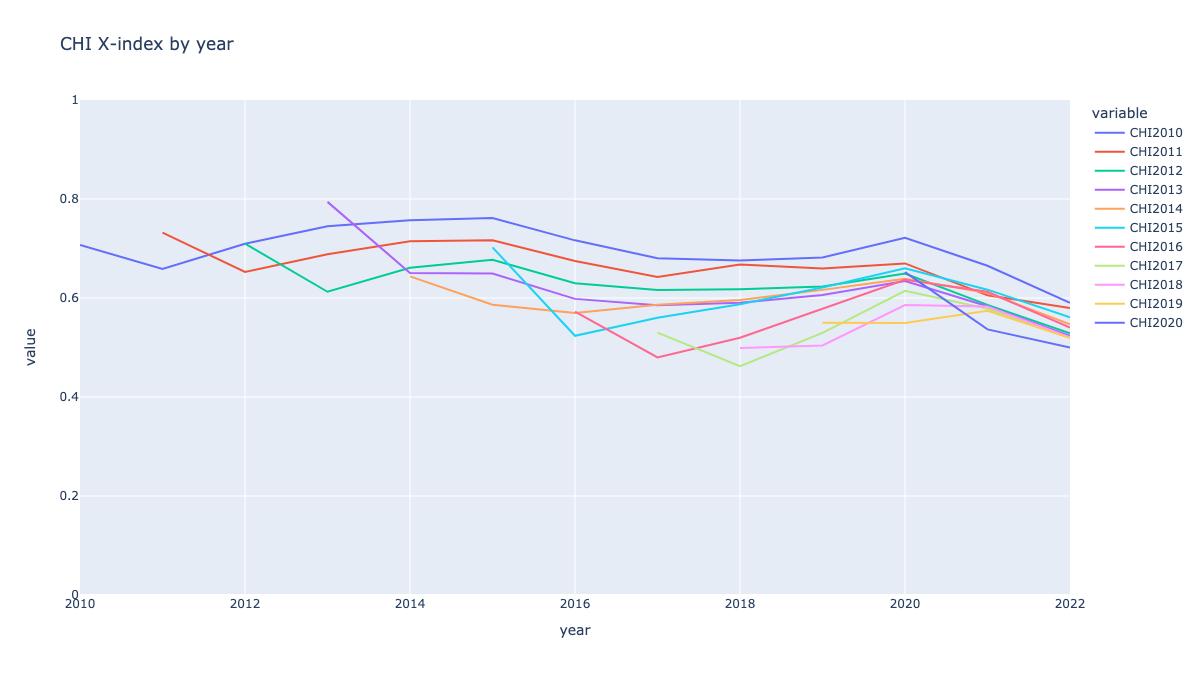
\includegraphics[width=\columnwidth]{figures/fig3_CHI.png}
    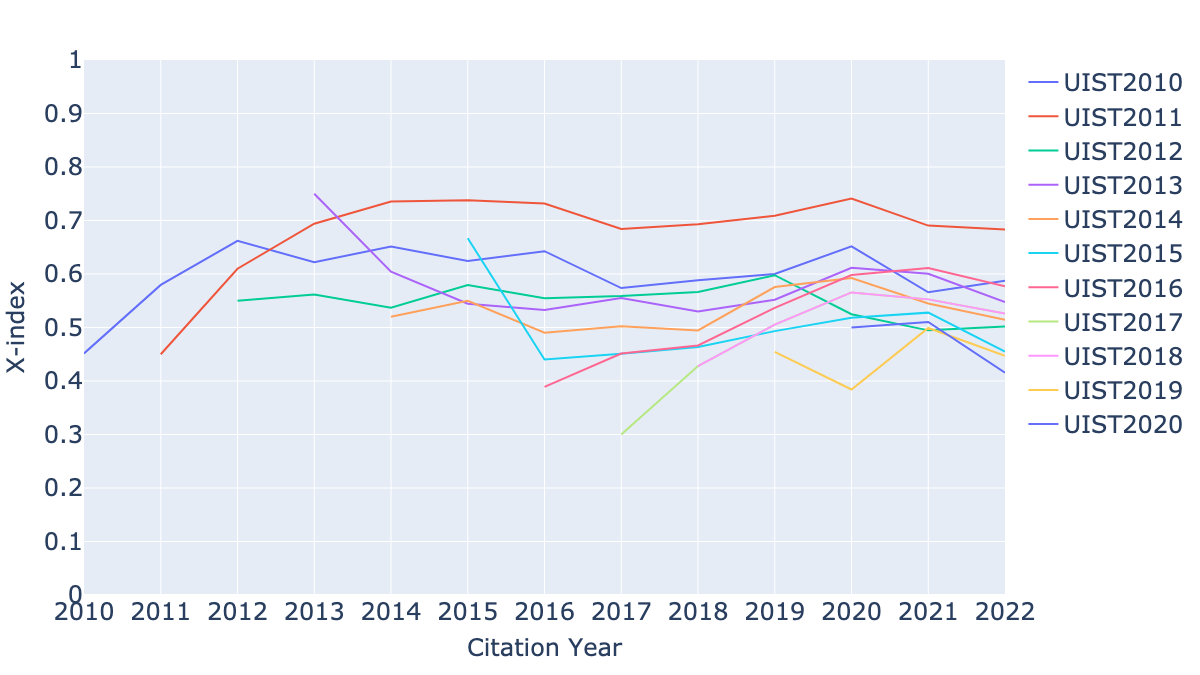
\includegraphics[width=\columnwidth]{figures/fig3_UIST.png}
    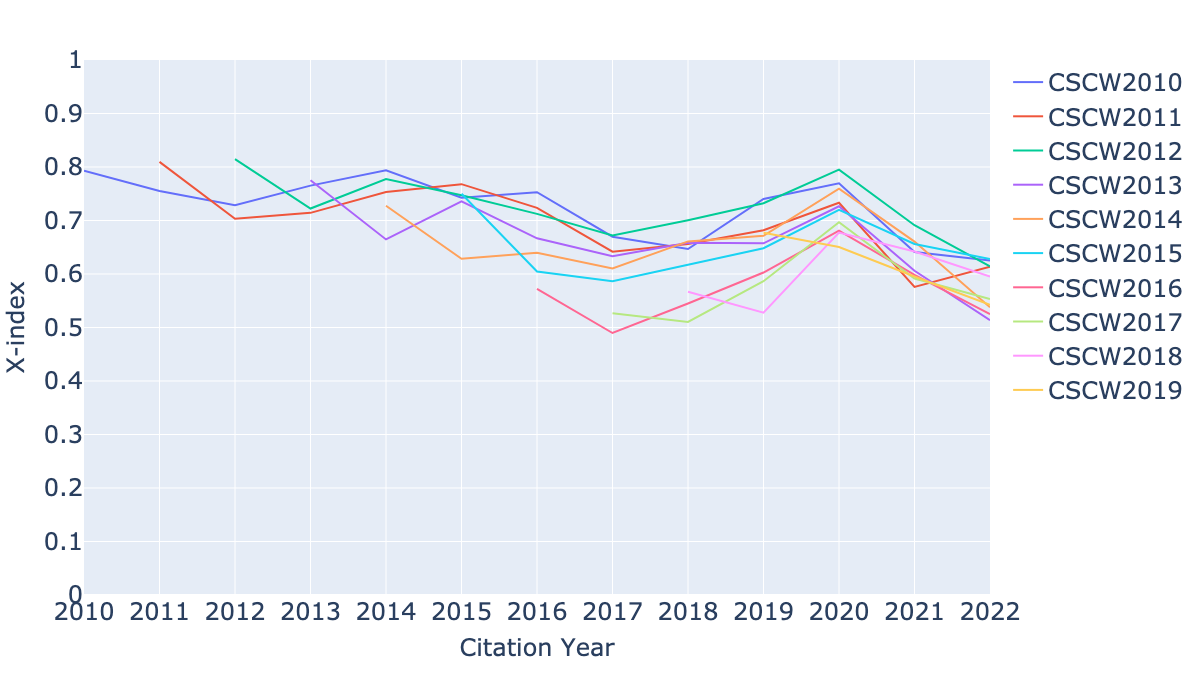
\includegraphics[width=\columnwidth]{figures/fig3_CSCW.png}
    \caption{.}
    \label{fg:fig3}
\end{figure}

\subsection{\xin Based on Each Year's Citations of HCI Papers}

The previous analysis suggests that we can aggregate each year's citations of HCI papers so that we can see how the non-HCI papers' interest in citing HCI papers changed over the years.

For each year, we consider that year's citations of HCI papers published in previous five years.
Since our HCI papers start earliest in 2010, our analysis can only begin from 2015 (A 2014 paper might cite a CHI 2009 paper but we do not have CHI 2009's citation information in our dataset).

\fgref{fig4} shows the results, which also exhibit a decreasing pattern over the years.
In other words, in the more recent years, HCI papers seem less likely to be cited by papers outside of our core HCI venue list.

\fg{fig4}{fig4}{1.0}{.}
\section{Discussion}

alternative interpretation
- maybe hci becomes more interdisciplinary
% \section{Implementation}
% \section{User Study}
% state the purpose ("To understand how xxx enables users to do yyy ...") and or research questions

\subsection{Tasks \& Procedure}
% tasks: what do you ask participants to do?

% procedure: besides the tasks, what other things happen in the order they happen (e.g., intro to the study -> tutorial/practice -> the task -> interview)

\subsection{Participants}
% report the # of participants, their age, gender, profession, and other relevant info.

% include:
% if there is a screening survey, briefly summarize the responses
% how do you recruit them?
% how much do you pay them?

\subsection{Apparatus}
% what software/hardware do you use for the study?

\subsection{Measurement}
% what metrics do you measure and how?

\subsection{Analyses, Results, \& Findings}
% how do you analyze the data?

% a brief summary of the results

% detailed reports of the results/findings
% - quantitative results grouped by metrics/measurements
% - qualitative results grouped by themes

% \section{Discussions}
% \section{Conclusion}

% Remove this citation later: \cite{bush1945we}.

\bibliographystyle{ACM-Reference-Format}
\bibliography{ref_main}

\end{document}